%!TEX root = paper.tex
In order to evaluate the applicability of PAC search to BitTorrent we conducted a measurement study of public BitTorrent networks. In order to evaluate PAC search over BitTorrent it is necessary to know: (i) how many nodes are in the network and (ii) how torrents are distributed over those nodes.

\subsection{Design}

    The data was collected from public BitTorrent trackers discovered using the TrackOn\footnote{\url{http://www.trackon.org}} API. Using the API we gathered a list of online public trackers. Public BitTorrent trackers are public facing trackers that place few restrictions on use. Any torrent can be registered at the tracker and any BitTorrent node can communicate with it. Each tracker was periodically polled with a \emph{scrape} request. A scrape request asks the tracker to return a list of all of the torrents that it is tracking. For each torrent in the scraped list, the tracker was asked to list all of the nodes that were currently sharing that torrent's file.

    This process was initiated at most once an hour. In practise a complete scrape took much longer than an hour to complete so additional scrapes were only started when the previous finished. Nodes were identified by IP address, it was assumed that each unique IP address represents a unique node and that every node has a single, unchanging IP address. This means that we cannot tell the difference between nodes that operate behind network address translation (NAT) and so may, as a result, undercount the number of nodes. We also cannot distinguish between nodes that share an IP address, for instance if an ISP reallocates an IP address to a different node. Again, this means that we undercount the number of nodes. We assume that these issues impact only slightly on our figures.

\subsection{Results}

    Between 1$^{\textrm{st}}$ May and 3$^{\textrm{rd}}$ July 2012, 13 public BitTorrent trackers were periodically scraped\footnote{Those trackers were:\\
        \url{http://bttrack.9you.com}\\
        \url{http://exodus.desync.com:6969}\\
        \url{http:/announce.xxx-tracker.com:2710}\\
        \url{http://h33t.com:3310}\\
        \url{http://bt.rghost.net}\\
        \url{http://61.154.116.205:8000}\\
        \url{http://fr33dom.h33t.com:3310}\\
        \url{http://announce.opensharing.org:2710}\\
        \url{http://bttrack.9you.com:8080}\\
        \url{http://tracker.torrentbay.to:6969}\\
        \url{http://bigtorrent.org:2710}\\
        \url{http://tracker.coppersurfer.tk:6969}\\
        \url{http://a.tv.tracker.prq.to}
    }. A total of 1.6 million distinct torrents were observed on over 5.4 million distinct nodes over 64 days. Considering each torrent as a document in the collection, the number of documents, $m=1,600,000$ and the number of nodes $n=5,400,000$. A PAC search is heavily influenced by the distribution of torrents over the nodes. In order to determine this distribution, the number of nodes registered to each torrent was counted. The frequencies at which these counts were observed was then calculated. Figure~\ref{fig:dist} shows these frequencies on a log-log scale, along with a line of best fit. The distribution follows a power law with the vast majority of torrents being found on very few nodes. These figures align roughly with those observed in \cite{guo_measurements_2005,dan_power-law_2010}. The analysis shows that 25\% of all torrents are only found on a single node and 76\% of all torrents are found on 10 or fewer. Only 2\% of observed torrents were found on more than 100 nodes. Torrents were found on anywhere between 0 and 21,445 nodes, the average torrent was owned by 27 nodes and the median torrent by 3. We saw in Section~\ref{sec:background} that documents needed to be replicated on tens of thousands of nodes in order to have a high probability of successful search. We observe that very few torrents meet those requirements. For a required probability of finding a document, $P(d_i)=0.8$ when querying $z=500$ nodes we need a document to be replicated on $r_i=17,354$ nodes. We only observed 9 torrents with a replication at or above this level.

    \begin{figure*}[t]
        \centering
        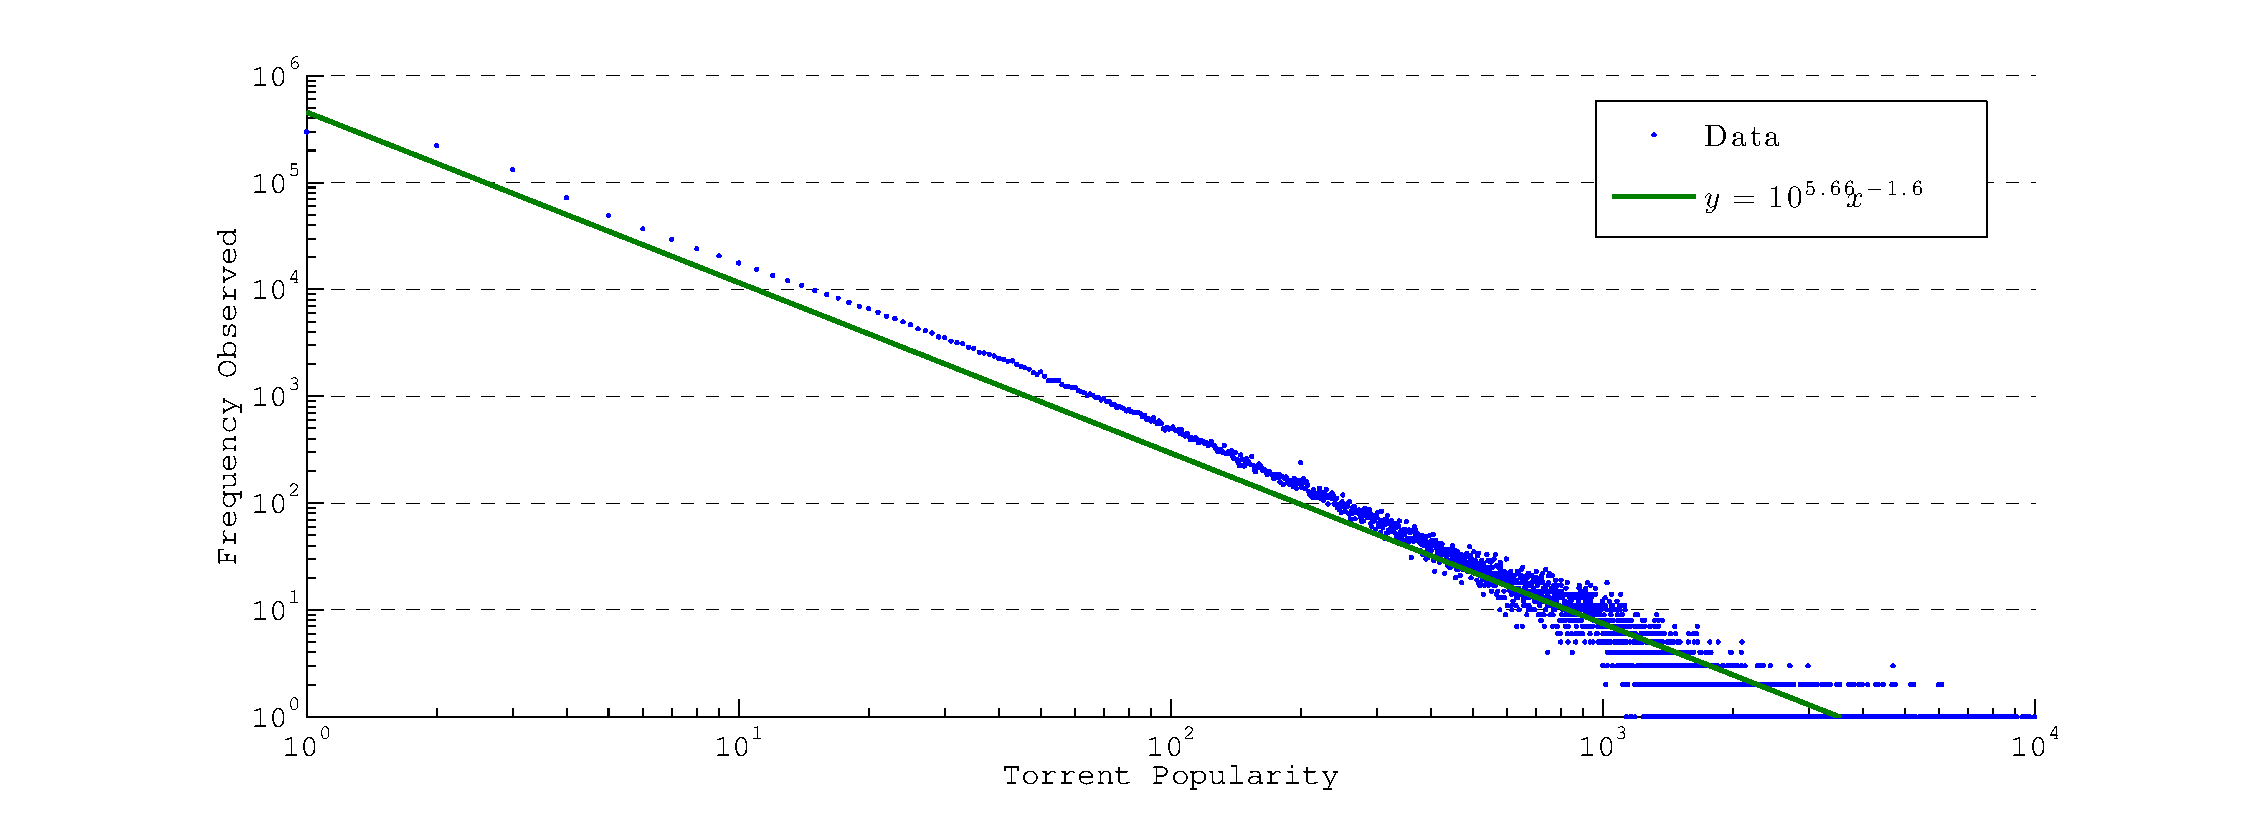
\includegraphics[width=0.8\textwidth]{Images/naturalDistribution.eps}
        \caption{The relative frequency of observations of torrent participation, i.e. the number of nodes that are downloading or uploading the torrent}
        \label{fig:dist}
    \end{figure*}
